\documentclass[12pt,oneside]{exam}

% This package simply sets the margins to be 1 inch.
\usepackage[margin=1in]{geometry}

% These packages include nice commands from AMS-LaTeX
\usepackage{amssymb,amsmath,amsthm,amsfonts,latexsym,verbatim,xspace,setspace}
\usepackage{hyperref}
\usepackage{graphicx}

% Make the space between lines slightly more
% generous than normal single spacing, but compensate
% so that the spacing between rows of matrices still
% looks normal.  Note that 1.1=1/.9090909...
\renewcommand{\baselinestretch}{1.1}
\renewcommand{\arraystretch}{.91}

% Define environments for exercises.
\newenvironment{exercise}[1]{\vspace{.1in}\noindent\textbf{Problem #1 \hspace{.05em}}}{}
\newenvironment{newsolution}{\vspace{.1in}\noindent\textbf{Solution: \hspace{.05em}}}{}

% define shortcut commands for commonly used symbols
\newcommand{\R}{\mathbb{R}}
\newcommand{\C}{\mathbb{C}}
\newcommand{\Z}{\mathbb{Z}}
\newcommand{\Q}{\mathbb{Q}}
\newcommand{\N}{\mathbb{N}}
\newcommand{\calP}{\mathcal{P}}
\DeclareMathOperator{\sech}{sech}
\DeclareMathOperator{\csch}{csch}
\DeclareMathOperator{\vsspan}{span}

\title{Math 514 - Summer II 2020: Homework 1}

%%%%%%%%%%%%%%%%%%%%%%%%%%%%%%%%%%%%%%%%%%

\begin{document}

\begin{flushright}
\sc MAT 514 - Summer II 2020\\
July 14, 2020
\end{flushright}
\bigskip
 
\begin{center}
\textsf{Solutions to Homework 1} 
\end{center}

%%%%%%%%%%%%%%%%%%%%%%%%%%%%%%%%%%%%%%%%

\begin{exercise}{1.1(e)}
 Given $z = (1+2i)$, compute 
\begin{equation*}
z^2+\overline{z}+i.
\end{equation*}
\end{exercise}

\noindent \textbf{Solution:} Direct computation leads to 
\begin{align*}
z^2 + \overline{z}+1 & = (1+2i)^2+(1-2i) + i \\
& = (1+4i-4) +(1-2i) + i\\
& = -2+3i.
\end{align*}

\vspace{1cm}

\begin{exercise}{1.2(c)}
Find the real and imaginary parts of 
\begin{equation*}
\left(\frac{-1+i\sqrt{3}}{2}\right)^3.
\end{equation*}
\end{exercise}


\noindent \textbf{Solution:} There are two ways of going about this problem. One is to perform the multiplications directly, the other to use properties of complex multiplication in polar form. Let's explore the second alternative. The polar form of $\frac{-1+i\sqrt{3}}{2}$ is 
\begin{equation*}
\frac{-1+i\sqrt{3}}{2} = 1\left[\cos\left( \frac{2\pi}{3} \right) + i \sin\left( \frac{2\pi}{3} \right)\right].
\end{equation*}
Multiplication in polar form multiplies the norms and adds the polar angles, so the polar form of $\left(\frac{-1+i\sqrt{3}}{2}\right)^3$ is 
\begin{equation*}
\left(\frac{-1+i\sqrt{3}}{2}\right)^3=  \cos(2\pi) + i\sin(2\pi) = 1, 
\end{equation*}
hence the desired real and imaginary parts are $1$ and $0$, respectively. 

\vspace{1cm}

\begin{exercise}{1.3(d)}
find the absolute value and conjugate of $(1+i)^6$. 
\end{exercise}

\noindent \textbf{Solution:} Let's simplify the problem by computing the exponentiation, 
\begin{align*}
(1+i)^6 & = [(1+i)^2]^3 \\
& = [(1+2i-1)]^3 \\
& = (2i)^3\\
& = -8i.
\end{align*}
The complex 
Its complex conjugate is $8i$, and the norm is $8$. 

\vspace{1cm}

\begin{exercise}{1.4.(h)}
Write 
\begin{equation*}
\left( \frac{1-i}{\sqrt{3}} \right)^4
\end{equation*}
in polar form.
\end{exercise}

\noindent \textbf{Solution:} We can simplify the problem by exponentiation, 
\begin{align*}
\left( \frac{1-i}{\sqrt{3}} \right)^4 & = \frac{(-2i)^2)}{9} \\
& = -\frac{4}{9}.
\end{align*}
The polar form is thus 
\begin{equation*}
\left( \frac{1-i}{\sqrt{3}} \right)^4 = \frac{4}{9}(\cos(\pi)+ i \sin(\pi)). 
\end{equation*}

\vspace{1cm}

\begin{exercise}{1.5(a)}
Write in rectangular for
\begin{equation*}
\sqrt{2}e^{i\frac{3\pi}{4}}.
\end{equation*}
\end{exercise}

\noindent \textbf{Solution:} This number is expressed using the complex exponential notation. Converting between it and rectangular form leads to
\begin{align*}
\sqrt{2}e^{i\frac{3\pi}{4}} & = \sqrt{2} \left[ \cos \left(\frac{3\pi}{4}\right) + i\sin \left( \frac{3\pi}{4}\right) \right] \\
& = \sqrt{2} \left[ -\frac{\sqrt{2}}{2} + i \frac{\sqrt{2}}{2} \right] \\
& = -1 + i.
\end{align*}

\vspace{1cm}

\begin{exercise}{1.9}
Find all solutions of the equation
\begin{equation*}
z^2+2z+(1-i) = 0.
\end{equation*}
\end{exercise}

\noindent \textbf{Solution:} The equation is simpler in the perfect square form
\begin{equation*}
z^2+2z+1 = i \Rightarrow (z+1)^2 = i
\end{equation*}
which can be easliy solved in terms of $\sqrt{i}$, 
\begin{equation*}
z_1 = -1+\sqrt{i}, \, z_2 = -1-\sqrt{i}.
\end{equation*}
In order to express these complex numbers in rectangular form, we need to compute $\sqrt{i}$. This is easliy done in polar form, 
\begin{equation*}
i = \cos\left(\frac{\pi}{2}\right) + i\sin \left(\frac{\pi}{2}\right),
\end{equation*}
so 
\begin{align*}
\sqrt{i} & = \cos\left( \frac{\pi}{4} \right) + i\sin \left( \frac{\pi}{4} \right) \\
& = \frac{\sqrt{2}}{2} + i \frac{\sqrt{2}}{2}.
\end{align*}
The solutions $z_1$ and $z_2$ can thus be written in rectangular form as
\begin{align*}
z_1 & = \left(-1+\frac{\sqrt{2}}{2}\right) + i \frac{\sqrt{2}}{2},\\
z_2 & = \left(-1-\frac{\sqrt{2}}{2}\right) - i\frac{\sqrt{2}}{2}.
\end{align*}

\vspace{1cm}

\begin{exercise}{1.11(d)}
Find all solutions to the equation $z^6-z^3-2=0$. 
\end{exercise}

\noindent \textbf{Solution:} The substitution $w=z^3$ simplifies the equation into a quadratic on $w$, 
\begin{equation*}
z^6-z^3-2 = w^2-w-2 = 0.
\end{equation*}
The solutions to this equaiton on $w$ are $w_1 =2$, $w_2 = -1$. To find the solutions in terms of $z$, we need to find their (complex) cubic roots. This is simpler in polar form. One way of representing $w_1$ is
\begin{equation*}
2 = 2[\cos(0) + i\sin(0)],
\end{equation*}
which leads to solutions
\begin{align*}
z_1 & = \sqrt[3]{2} \left[\cos(0) + i\sin(0)  \right] \\
z_2 & = \sqrt[3]{2} \left[ \cos \left(\frac{2\pi}{3}\right)+i\sin\left(\frac{2\pi}{3} \right)\right]  \\
z_3 & = \sqrt[3]{2} \left[ \cos \left(\frac{4\pi}{3}\right) + i \sin \left(\frac{4\pi}{3}\right) \right].
\end{align*}
Meanwhile, $w_2=-1$ can be written in polar form as 
\begin{equation*}
-1 = \cos(\pi)+i\sin(\pi).
\end{equation*}
This leads to the solutions
\begin{align*}
z_4 & = \cos(\pi)+i\sin(\pi) \\
z_5 & = \cos\left( \frac{\pi}{3}\right)+ i \sin \left( \frac{\pi}{3}\right) \\
z_6 & = \cos \left( \frac{5\pi}{3} \right) + i \sin\left(\frac{5\pi}{3}\right).
\end{align*}

\vspace{1cm}

\begin{exercise}{1.29}
Let $G$ be the set of points $z \in \mathbb{C}$ satisfying: either $z$ is real and $-2 < z < -1$, or $|z|<1$, or $z=1$, or $z=2$.
\begin{itemize}
\item[(a)] Sketch the set $G$, being careful to indicate exactly the points that are in $G$. 
\item[(b)] Determine the interior points of $G$.
\item[(c)] Determine the boundary points of $G$.
\item[(d)] Determine the isolated points of $G$.
\end{itemize}
\end{exercise}

\vspace{0.5cm}

\noindent \textbf{Solution:}
\begin{itemize}
\item[(a)] The plot of the region is outlined below

\begin{center}
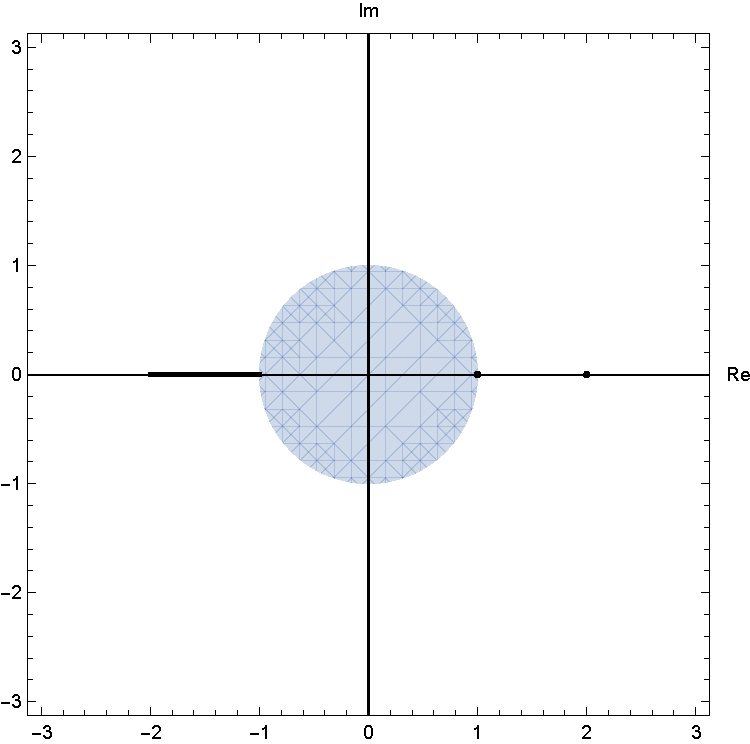
\includegraphics[scale=0.5]{p1.pdf}
\end{center}


\item[(b)] 
\begin{equation*}
\mathring{G} = \{z \in \mathbb{C} | |z|<1\}
\end{equation*}
\item[(c)] 
\begin{equation*}
\partial G = \{z \in \mathbb{C} | |z| =1\} \cup \{ z \in \mathbb{C} | \Im(z) =0, \mbox{and} \, -2 \leq z \leq -1\}
\end{equation*}
\item[(d)] The only isolated point of $G$ is $z=2$.
\end{itemize}

\vspace{1cm}

\begin{exercise}{1.33}
Find a parametrization for each of the following paths:
\begin{itemize}
\item[(a)] the circle $C[(1+i,1]$, oriented counter-clockwise;
\item[(b)] the line segment from $(-1-i0$ to $wi$;
\item[(c)] the top half of the circle $C[0,34]$;
\item[(d)] the rectangle with vertices $\pm 1 \pm 2i$, oriented counter-clockwise;
\item[(e)] the ellipse 
\begin{equation*}
\{z \in \mathbb{C} | \, |z-1|+|z+1|=4\}
\end{equation*}
oriented counter-clockwise.
\end{itemize}
\end{exercise}

\vspace{0.5cm}

\noindent \textbf{Solution:} 
\begin{itemize}
\item[(a)] 
\begin{equation*}
\alpha(t) = 1+i + e^{it},
\end{equation*}
for $0 \leq t \leq 2\pi$.
\item[(b)] 
\begin{equation*}
\beta(t) = (-1-i)91-t)+2ti,
\end{equation*}
for $0 \leq t \leq 1$.
\item[(c)] 
\begin{equation*}
\gamma(t) = 34e^{i(\pi-t)}, 
\end{equation*}
for $0 \leq t \leq \pi$.
\item[(d)] 
\begin{equation*}
\delta(t) = \left\{ 
\begin{array}{rl}
(1+2i)(1-t)+(-1+2i)t, & \, \mbox{for} \, 0 \leq t \leq 1,\\
(-1+2i)(2-t)+(-1-2i)(t-1), & \, \mbox{for} \, 1 \leq t \leq 2,\\
(-1-2i)(3-t)+(1-2i)(t-2), & \, \mbox{for} \, 2 \leq t \leq 3,\\
(1-2i)(4-t) + (1+2i)(t-3), & \, \mbox{for} \, 3 \leq t \leq 4
\end{array}
\right.
\end{equation*}
\item[(e)] This is an ellipse with major axis along the real axis, with length $4$, and minor axis along the imaginary axis, with length $2\sqrt{3}$. It can be parametrized by 
\begin{equation*}
\epsilon(t) = 2\cos(t)+i\sqrt{3}\sin(t),
\end{equation*}
for $0 \leq t \leq 2\pi$.
\end{itemize}
\end{document}

